\documentclass[12pt]{article}
\usepackage[a4paper, total={17cm, 23cm}]{geometry}
\usepackage{graphicx}
\usepackage{titlesec}
\usepackage{setspace}
\usepackage{listings}
\usepackage{tikz}
\usepackage{lmodern} % for bold teletype font
\usepackage{xcolor}
\usepackage{hyperref}
\usepackage{glossaries}
\usepackage[portuguese]{babel}
\usepackage{float}
\usepackage{courier}
\usepackage{tcolorbox}
\usepackage{booktabs}
\usepackage{array}
\usepackage{indentfirst} % Garante a correta indentação do primeiro parágrafo de cada secção

% ----------- CONFIGURAÇÕES PACKAGES ----------- %

\hypersetup{
    colorlinks=true,
    linkcolor=black,
    linkbordercolor = {white},
}

\definecolor{codeBlue}{rgb}{0.2,0.2,1}
\definecolor{codeGreen}{rgb}{0,0.5,0}
\definecolor{codeRed}{rgb}{0.9,0,0}
\definecolor{CodeGrey}{rgb}{0.46,0.45,0.48}
\definecolor{backcolour}{rgb}{0.95,0.95,0.92}

\lstset{ %Linguagem
    showspaces=false,
    showtabs=false,
    breaklines=true,
    showstringspaces=false,
    captionpos=b,
    keepspaces=true,
    numbersep=5pt,
    breakatwhitespace=true,
    postbreak=\mbox{\textcolor{red}{$\hookrightarrow$}\space},
    basicstyle=\footnotesize,
    commentstyle=\color{codeGreen},
    keywordstyle=\color{codeBlue} \ttfamily\small,
    stringstyle=\color{codeGreen},
    linewidth=15cm
}

\titleformat{\section}{\normalfont\large\bfseries\raggedright}{\thesection}{1em}{}
\titleformat{\subsection}{\normalfont\normalsize\bfseries\raggedright}{\thesubsection}{1em}{}
\titleformat{\subsubsection}{\normalfont\normalsize\bfseries\raggedright}{\thesubsubsection}{1em}{}



%Graphic path
\graphicspath{ {Resourcers/} }

% ----------- CONFIGURAÇÕES PACKAGES ----------- %

% ----------- CONFIGURAÇÕES VARIAVEIS ----------- %

\def\logoEscola{logoIpt.png} %Logo da Escola
\def\local{Local} %Local
\def\curso{Engenharia Informática} %Curso
\def\escola{Instituto Politécnico de Tomar} %Escola
\def\autor{Afonso Viana \& Igor Fonseca} %Autor relatório
\def\titulo{Trabalho Prático} %Título do documento

%Estagio
\def\localEstagio{Local estagio (Opcional)} %Local do estágio
\def\instEstagio{Instituto do estagio (Opcional)} %Instituição do estágio

% ----------- FIM CONFIGURAÇÕES VARIAVEIS ----------- %

% Configuração do título
\title{\textbf{\titulo}}
\author{\Large \autor \vspace{0.3cm}}

\begin{document}

% ---------- FUNÇÕES --------- %

\newcommand{\forceIndent}{\hspace{\parindent}}

% ---------- FIM FUNÇÕES --------- %

% ----------- CAPA RELATORIO----------- %

%Título documento
\maketitle

%LOGO no canto superior esquerdo
\begin{tikzpicture}[remember picture,overlay]
	\node[anchor=north west,yshift=-1.5pt,xshift=1pt]%
	at (current page.north west)
	{\includegraphics[scale=0.5]{\logoEscola}};
\end{tikzpicture}

\vspace{6cm}
\par
\large\centering \curso
\vspace{2mm}
\par
\normalsize \escola

\pagenumbering{gobble}

% ---- Opcional, informações de estágio ---- %

%\newpage
%\begin{tikzpicture}[remember picture,overlay]
%    \node[anchor=north west,yshift=-1.5pt,xshift=1pt]%
%    at (current page.north west)
%    {\includegraphics[scale=0.5]{\logoEscola}};
% \end{tikzpicture}

%Local estágio caso necessário
%\vspace{2cm}
%\Large\textbf{\localEstagio} \par
%\large \instEstagio

% ---- Opcional, informações de estágio ---- %

% ------------------ FIM CAPA RELATORIO----------------- %

% ---- Opcional, contextualização de documento ---- %

%\newpage

%\raggedleft\small\emph{Relatório de estágio apresentado no Instituto Politécnico de Tomar}
%\par
%\raggedleft\small\emph{para cumprimento dos requisitos necessários à obtenção do grau}
%\par
%\small\emph{Pós-secundário em Informática}

% ---- Fim Contextualização de documento ---- %

% ----------- DESENVOLVIMENTO RELATORIO----------- %

% -- CONFIGURAÇÕES CONTEÚDO -- %

%gerais
\raggedright
\setlength\parindent{24pt}
\renewcommand{\baselinestretch}{1.2}

% Indice
\newpage
\tableofcontents

\newpage
\renewcommand{\listfigurename}{Lista de figuras}
\listoffigures

\newpage
\section{Introdução}
O presente relatório descreve o desenvolvimento da plataforma SkillBridge, uma aplicação Web cujo objetivo é facilitar a aproximação entre estudantes/profissionais e empresas através da promoção de experiências de job shadowing.
\par O job shadowing consiste numa prática em que um indivíduo acompanha, durante um curto período de tempo, um profissional no exercício das suas funções, permitindo conhecer de forma prática a realidade de uma determinada profissão ou área de atividade. A plataforma SkillBridge surge como resposta à necessidade de criar um ponto de encontro digital entre quem procura este tipo de experiência e as empresas/profissionais dispostos a proporcioná-la, simplificando todo o processo de divulgação, candidatura e gestão destas oportunidades.
\par A aplicação foi desenvolvida com recurso a ASP.NET Core MVC e Razor Pages, utilizando Entity Framework e LINQ para o acesso e manipulação dos dados, e SignalR para funcionalidades de comunicação em tempo real. O sistema permite a gestão de utilizadores com diferentes perfis de acesso, a publicação e candidatura a oportunidades de job shadowing, bem como a gestão de toda a informação associada, respeitando as operações fundamentais de criação, edição, eliminação e visualização de dados.
Ao longo deste relatório serão apresentadas as principais decisões tomadas durante o desenvolvimento, a arquitetura da aplicação, o modelo de dados implementado, as funcionalidades disponibilizadas, bem como os mecanismos de validação, segurança e controlo de acesso utilizados para garantir o correto funcionamento da plataforma.

\section{Desenvolvimento aplicacional}
\subsection{Estrutura Aplicacional}
\subsubsection{Arquiteturas}

\begin{table}[H]
\centering
\begin{tabular}{|l|l|}
\hline
\textbf{Componentes}   & \textbf{Tecnologia}                                 \\ \hline
Framework     & ASP.NET Core (.NET 10) + Razer Pages       \\ \hline
Autenticação  & ASP.NET Core Identity                      \\ \hline
Base de Dados & Entity Framework Core com SQL Server       \\ \hline
Websocket     & SignarR (Chat, Code Editor e Notificações) \\ \hline
Frontend      & Bootstrap e CSS modular por página         \\ \hline
\end{tabular}
\end{table}
\subsubsection{Conceito Base}
\begin{figure}[H]
    \begin{center}
        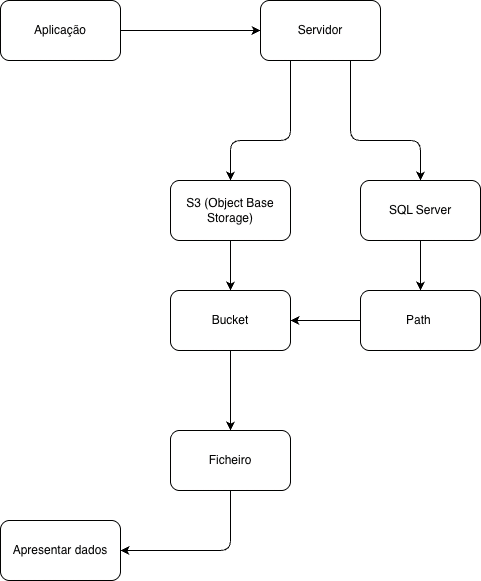
\includegraphics[scale=0.7]{fluxograma_aplicacional.png}
        \caption{Fluxograma aplicacional}
    \end{center}
\end{figure}

\subsubsection{Conceito Aplicado}
\begin{figure}[H]
    \begin{center}
        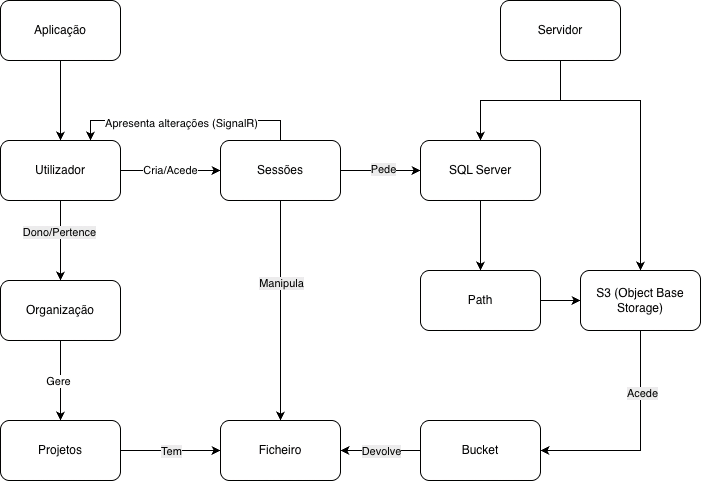
\includegraphics[scale=0.7]{aplicacao.png}
        \caption{Estrutura aplicacional}
    \end{center}
\end{figure}
\subsection{Características Aplicacionais e Funcionalidades}
O projeto \emph{Skillbridge} foi desenvolvido como uma plataforma Web destinada à gestão da intereção entre utilizadores e organizações, permitindo a publicação e gestão de oportunidades, bem como a administração dos diferentes recursos da aplicação.
\subsubsection{Gestão de Utilizadores}
A Aplicação implemente um sistema de autenticação baseado no \textbf{ASP.NET Core Identity}, permitindo o registo, autenticação e gestão de contas de utilizador.\\
Cada utilizador possui um perfil próprio, podendo aceder às funcionalidades disponíveis de acordo com o seu nível de permissões. O controlo de acesso é efetuado através de mecanismo de autorizações, restringido determinadas operações apenas a utilizadores autenticados ou administradores.
\subsubsection{Gestão de Organizações}
Uma das principais funcionalidades da plataforma consiste na gestão de organizações.\\
Qualquer utilizador autenticado por criar novas organizações, editar as respetivas informações e gerir os seus membros.\\
Durante o desenvolvimento foram ainda implementadas funcionalidades adicionais, tais como:
\begin{itemize}
    \item Promoção de membros
    \item Remoção de membros
    \item Atualizações das informações da organizações
    \item Controlo de permissões dos diferentes participantes
\end{itemize}
Foi também adicionado a possibilidade de associar imagens/logotipos às organizações, estas imagens iriam ser armazenadas num \emph{bucket} específico no serviço \textbf{Amazon S3}.
Estas funcionalidades sofreram diversas melhorias ao longo da evolução do projeto, conforme evidenciado pelo histórico de commits.
\subsubsection{Gestão de Membros}
Cada organização possui um conjunto de membros associados.\\
Foram desenvolvidas funcionalidades que permitem:
\begin{itemize}
    \item Adicionar novos membros
    \item Remover participantes
    \item Promover membros para funções administradoras
    \item Controlar as permissões de cada elemento
\end{itemize}
A implementação deste módulo permite uma gestão mais flexível das organizações existentes na plataforma, no entanto apenas é possível a promoção dos membros.
\subsubsection{FAQ}
Foi também criada uma secção (simulada) de \textbf{Perguntas Frequentes (FAQ)} destinada a esclarecer dúvidas existentes na plataforma. Esta funcionalidade iria melhorar significativamente a experiência caso aplicada num cenário real.
\subsubsection{Sistemas de Notificações}
Durante o desenvolvimento foram adicionadas notificações visuais destinadas a informar o utilizador sobre o resultado das diferentes operações. Entre estas operações encontram-se:
\begin{itemize}
    \item Confirmação de operação realizadas com sucesso
    \item Mensagem de erro
    \item Alertas informativos
    \item Diálogos de confirmação antes de operações
\end{itemize}
Estas funcionalidades melhoram a usabilidade da aplicação significativamente.
\subsection{Tratamento de Erros}
A aplicação possui páginas de erro personalizadas para diferentes situações.\\
Sempre que ocorre uma exceção ou um recurso não é encontrado, o utilizador é reencaminhado para páginas específicas, evitando a apresentação de mensagens técnicas do servidor.\\
Isto permite uma utilização segura e estável de forma a prevenir que o utilizador aceda a páginas "partidas" ou apresentação de erros aplicacionais.
\subsection{Segurança}
Durante o desenvolvimento da aplicação foram implementadas diversas medidas destinadas a aumentar a segurança da aplicação. Entre elas destacam-se:
\begin{itemize}
    \item Proteção \emph{Anti-Forgery} nos formulários, que preveni o uso de tokens da aplicação a partir de pedidos de outros aplicações menos fidedignas
    \item Validação de dados recebidos
    \item Controlo de permissões nas operações
    \item Autenticação baseada em \emph{Identity}
    \item Restrição de acesso a funcionalidades administrativas
\end{itemize}
Estas medidas reduzem significativamente o risco de ataques comuns em aplicações Web e a inserção de formato de dados errados que por sua vez poderiam danificar o funcionamente da aplicação.
\end{document}
